The system allows users to reserve available cars, to manage their requests and charge them for the rental.

The users can:
\begin{itemize}
\item Register to the service;
\item Login with their personal account;
\item Edit and manage personal information;
\item Delete their existing account;
\item Locate nearby available-to-rent vehicles;
\item Reserve one of said cars for a fixed amount of time;
\item Unlock the reserved vehicle based on their mobile device GPS position;
\item Alternatively, unlock the reserved car by inserting a vehicle-specific code (found on the windshield) into the application;
\item Start the engine by inserting their PIN;
%solo cose che può fare o anche informazioni che può ricevere? notifica parcheggi e spesa corrente
\item Perform payments for the used service via credit card or \emph{PayPal\textsuperscript{TM}}.
\end{itemize}
\begin{figure}[!h]
	\centering
		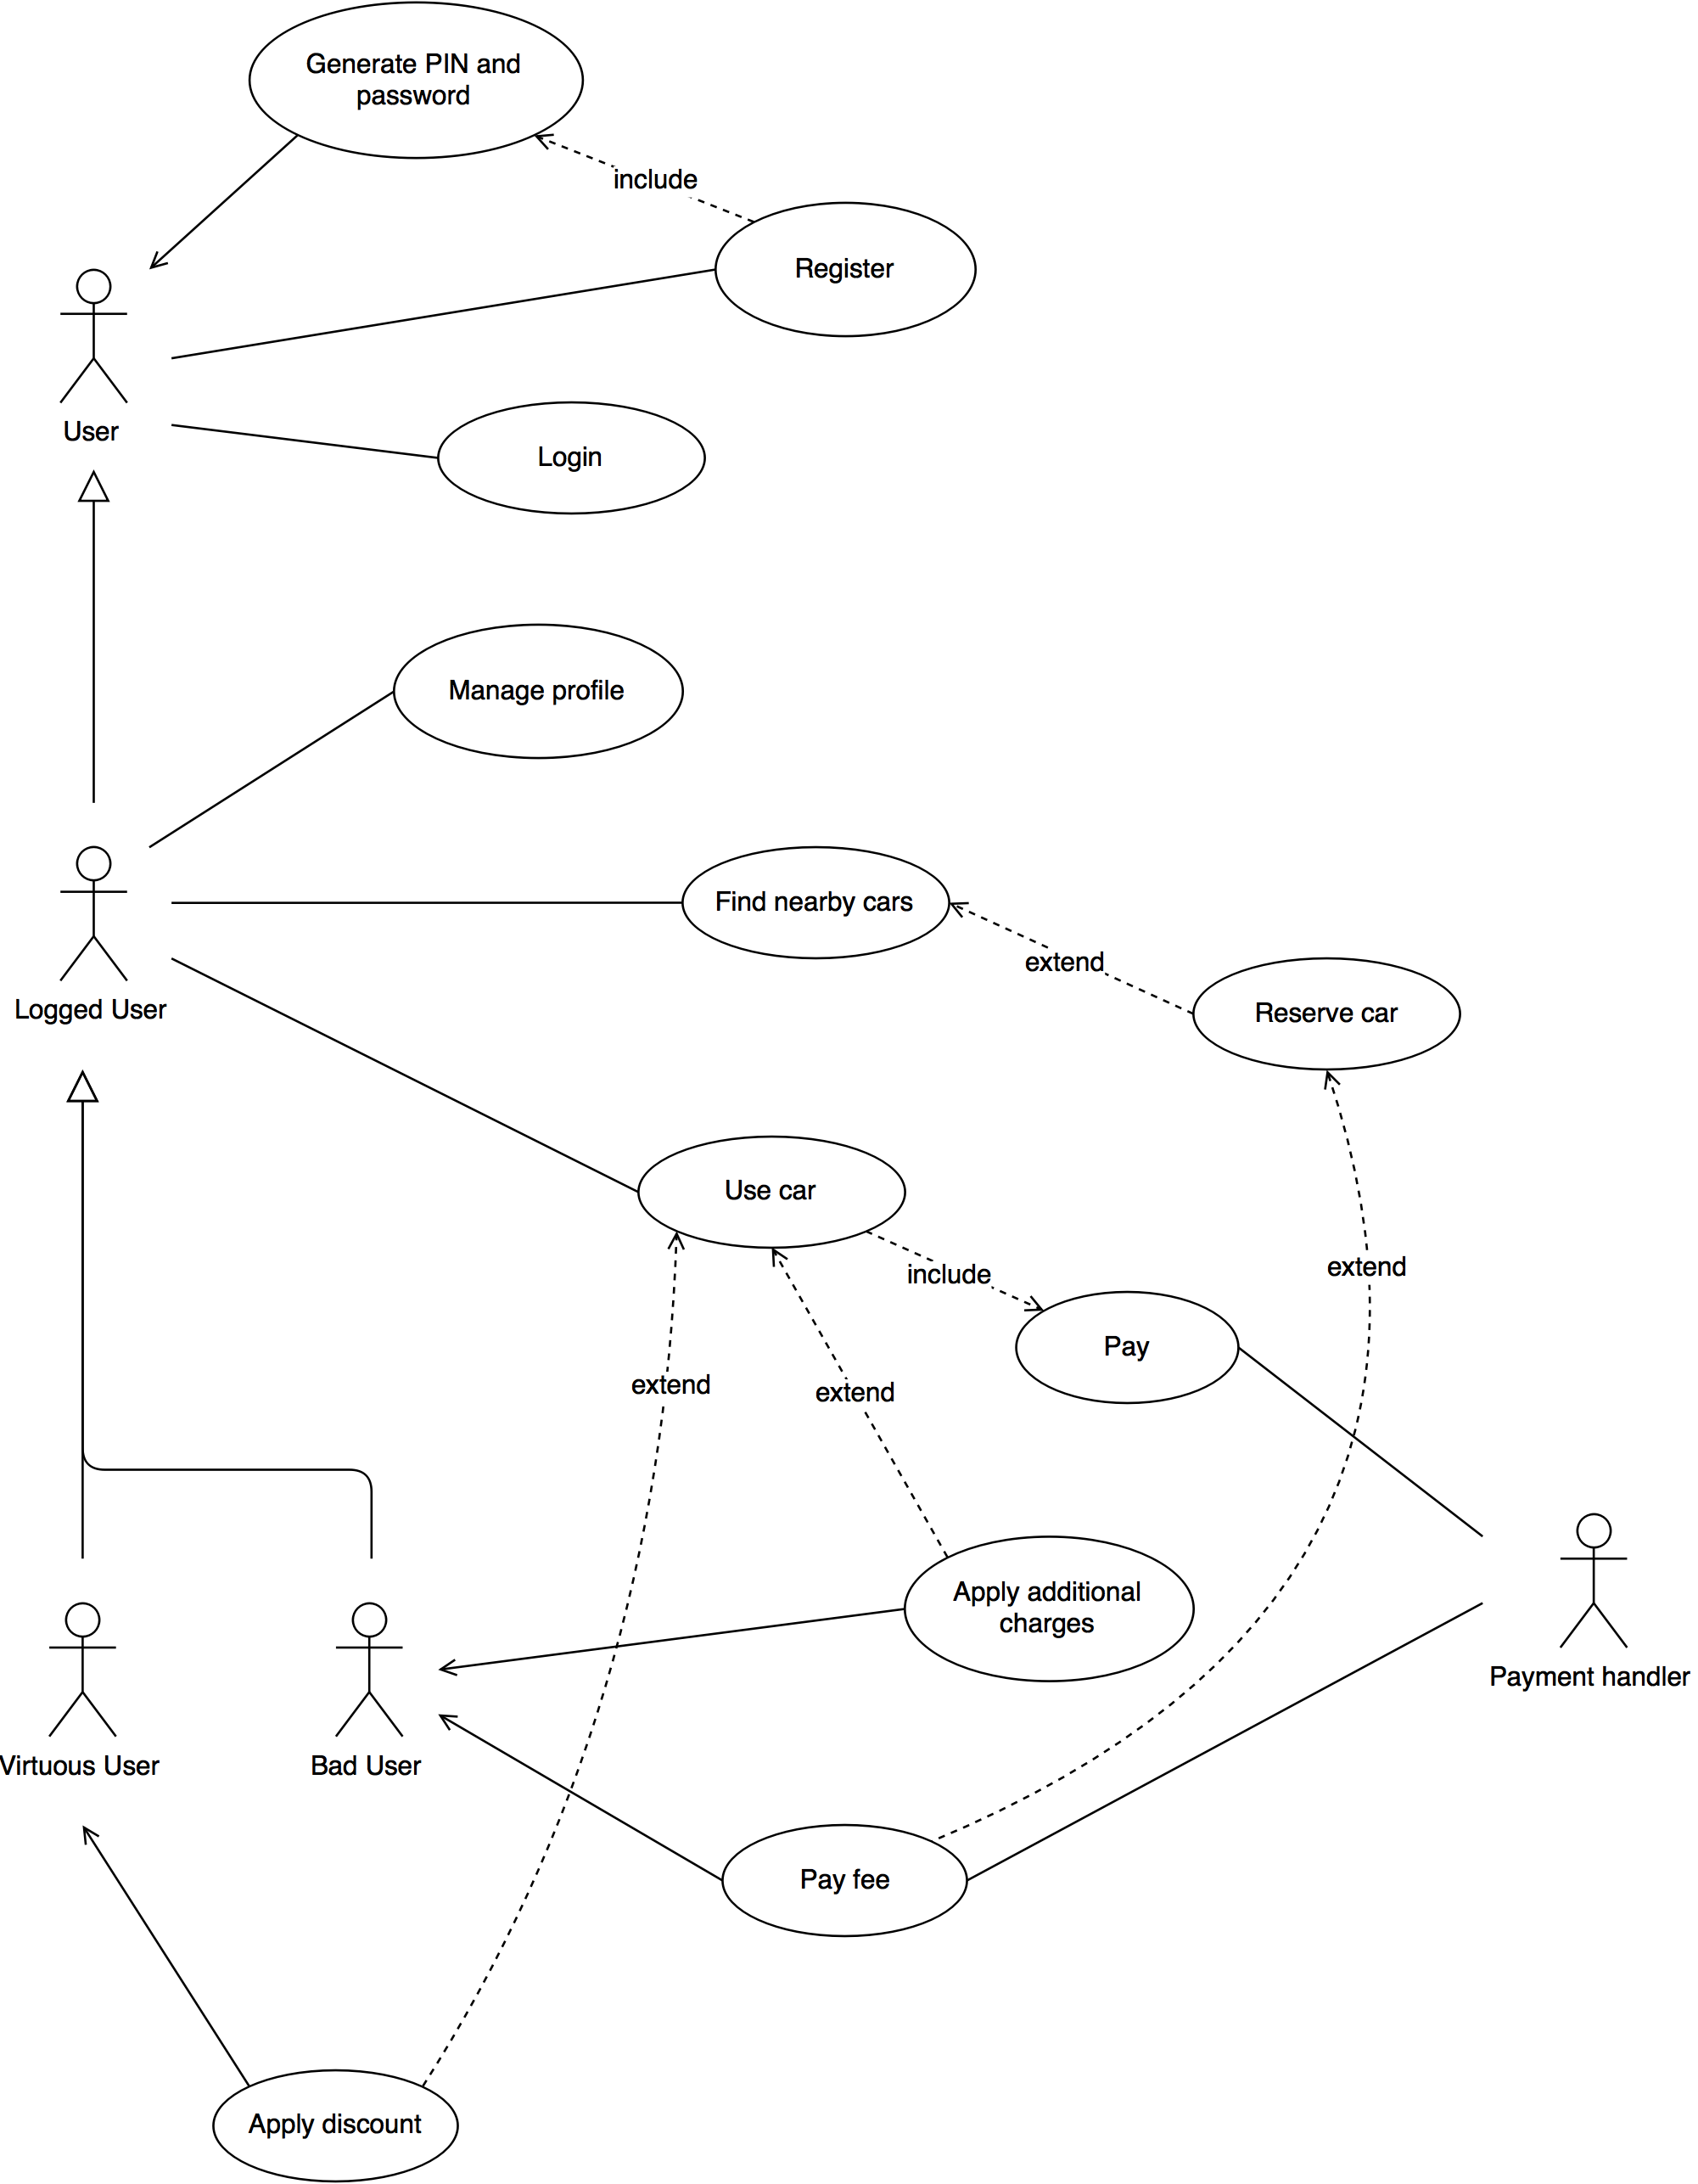
\includegraphics[width=\textwidth]{./pictures/use_case.png}
		\caption{The comprehensive use-case diagram of all the functionalities provided by the 						system}
\end{figure}